\chapter{Infraestructura}

Este capítulo recoge el conjunto de herramientas seleccionadas para este proyecto, así como una detallada descripción de la relación entre unas y otras que conformará la infraestructura del proyecto.
Se introducirá cada una de las herramientas y se especificará tanto las razones bajo la elección de la misma para el proyecto como la función que cumplirá en él.

\section{Herramientas utilizadas}

El presente apartado es el resultado de los meses de investigación, en los cuales estudiamos numerosas herramientas, entornos y plataformas aplicables a la robótica que podían aportar algo a nuestros intereses. Finalmente se escogieron los que se presentan a continuación para formar parte de la solución de ``Ejecución mixta'' para aplicaciones robóticas.

\subsection{Tecnologías Web}

En los primeros días de exploración salió rápidamente a la luz el entorno en el que debíamos acotar la búsqueda e investigación. Recordemos que el fin último es aumentar la accesibilidad de la robótica, y que en accesibilidad no existe ningún ámbito que supere a las tecnologías web. Algunos años atrás resultaba impensable plantear un desarrollo robótico empleando este tipo de tecnología dado que los motores web apenas tenían potencia de cómputo suficiente para reproducir un vídeo, y mucho menos podían si quiera superar los límites del navegador para acceder a dispositivos externos. Todo esto ha cambiado hasta tal punto en que se pueden crear aplicaciones tan exigentes como juegos en realidad virtual, procesamiento de imágenes, la comúnmente llamada ``minería de datos'' o KDD e incluso tareas de aprendizaje automático gracias a la habiliticación del acceso al \textit{hardware} de aceleración gráfica por parte del navegador y a la incorporación en el mismo de potentes núcleos o motores de ejecución, dando lugar a las aplicaciones dinámicas en la nube (Fig. \ref{web}).

\begin{figure}[!hbtp]  \centering\noindent
    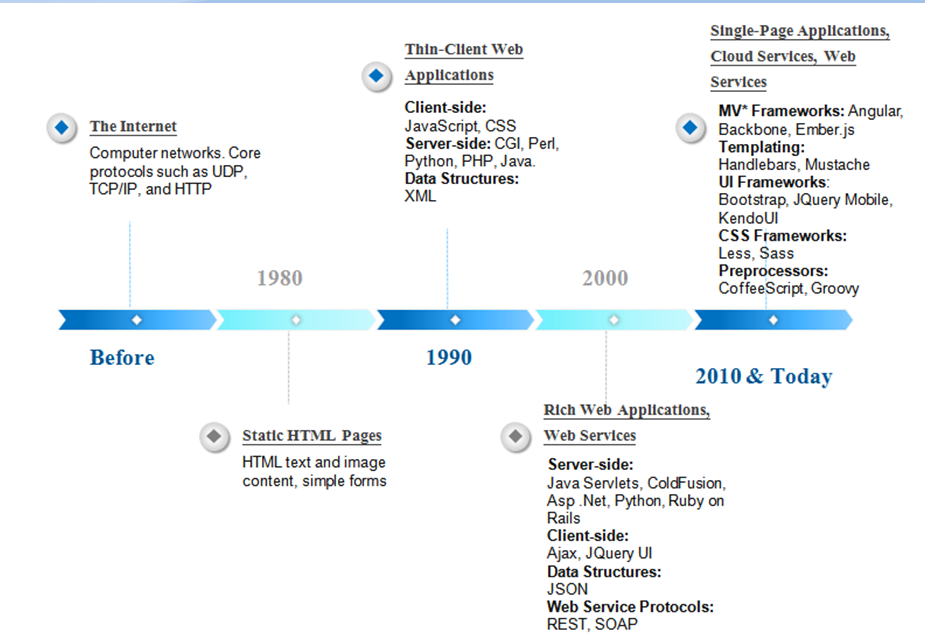
\includegraphics[width=0.99\textwidth]{figures/web-history.png}
    \caption{Evolución de las Tecnologías Web}
    \label{web}
\end{figure}

En la actualidad, se puede construir aplicaciones para casi cualquier caso de uso, incluido el de la robótica, completamente formados por herramientas web. Gran parte de sus ventajas residen en que el acceso a la web es totalmente público y sencillo, de tal manera que un servicio ofrecido a través de la web puede ser usado por cualquier persona del planeta, con independencia de su sistema operativo, dispositivo o entorno.

Dado que Internet no es más que un conjunto debidamente interconectado de sistemas y redes de sistemas que se comunican a través de protocolos conocidos (mirándose con un gran nivel de abstracción), se puede conseguir de manera bastante eficaz conectar herramientas de distinta naturaleza para que funcionen como un conjunto homogéneo a través de Internet. Precisamente por eso se escogió este tipo de tecnologías para establecer la base del proyecto, que nos permitirán conectar la parte cliente de la aplicación con el lado servidor para organizar un proceso de ejecución compartida utilizando protocolos preestablecidos que conozcan ambas partes, cumpliendo la función de mediador entre ellas y estableciendo la jerarquía que permita orquestar todo de manera transparente para el usuario.

Entre las funciones que nos ofrece la web, destacamos especialmente el acceso al \textit{hardware} del equipo cliente, el soporte de almacenamiento en la nube, los mecanismos de seguridad, las características de sus canales de comunicación (baja latencia punto a punto, retransmisiones, baja tasa de error y de paquetes perdidos,...) y la capacidad de ejecutar el código de la aplicación. Como se puede ver, todas ellas sirven para distintos tipos de tareas, de manera que no se puede decir que las tecnologías web formen una parte específica de este proyecto, sino más bien que actúan de base y ``pegamento'' para estructurar todas las que se exponen a continuación, además de facilitarnos un entorno de trabajo completo.

Por último, lo que hace ideal a la web para este proyecto es que su acceso, como ya se ha dicho, es a través de un navegador web. Este es el agente que tiene visibilidad tanto interna como externa, es decir, que puede comunicarse tanto con el PC o sistema en el que está instalado como con el resto del mundo. Los mecanismos básicos de seguridad de la red, como \textit{firewalls} y NATs no permiten ciertos tipos de comunicaciones que se consideran peligrosas, como aquellas que provienen de subredes externas o de sitios desconocidos. Con una aplicación remota no podemos actuar sobre el sistema del cliente, pero si podemos ``hablar'' con el navegador, que a su vez puede ejercer control sobre el sistema. En otras palabras, podemos utilizar el navegador como una especie de \textit{proxy} que redirija los mensajes específicos de nuestra aplicación a su destinatario, siempre y cuando éste tenga un interfaz web o sea accesible a través de ella.

\subsection{Proyecto Jupyter}

La herramienta fundamental en la que se basa este desarrollo es el proyecto Jupyter\footnote{\url{https://jupyter.org/}}, la evolución de \textit{IPython 3.0}. Se trata de una aplicación web de código abierto que ofrece la capacidad de crear y compartir documentos, llamados cuadernillos o \textit{Notebooks}, los cuales puede contener textos narrativos y elementos de texto enriquecido (párrafos, ecuaciones, figuras, enlaces, etc.), imágenes ilustrativas, códigos empotrados, ecuaciones, visualizaciones (figuras, gráficos, tablas, etc.) y gran cantidad de elementos gráficos inteligentes. La razón principal bajo su elección, además de por pertenecer al ámbito de las tecnologías web, es que además de empotrar y editar código el usuario puede ejecutarlo desde su navegador, gracias a la comunicación implícita de la aplicación con los núcleos o \textit{kernels} de computación que incluye el navegador, incluyendo intérpretes para distintos lenguajes. Con ello, se dispone de una herramienta a través de la cual se pueden llevar a cabo potentes tareas como la transformación de datos, el modelados estadístico de los mismos, simulaciones numéricas, visualización y análisis de los datos y aprendizaje automático, siendo todos ellos sus principales usos, aunque su funcionalidad es mucho más amplia.

La característica principal del entorno son sus \textit{Notebooks}, documentos generados a través del interfaz de usuarios que pueden contener todo lo anteriormente mencionado, completamente legibles por usuarios humanos pero con capacidad para ejecutar código de computadora en hasta 100 lenguajes diferentes para los que da soporte en la actualidad. Básicamente consisten en una
secuencia lineal de celdas que pueden ser de diferentes tipos, dependiendo de su contenido:
\begin{itemize}
\item Celdillas de código: entrada y salida del código en el lenguaje seleccionado para el \textit{Notebook} que se ejecuta en el \textit{kernel}. Estas celdas son extensibles para poder visualizar el resultado de la ejecución del código especificado.
\item Casillas de reducción: contienen texto narrativo con ecuaciones en formato LaTeX embebidas.
\item Encabezado de celdas: texto de 6 niveles de organización jerárquica y formato. Útiles para establecer títulos y subtítulos y obtener un documento mucho más claro y ordenado.
\item Celdas sin formato: texto sin formato específico para ser exportado a diferentes formatos mediante \textit{nbconvert} sin sufrir cambios.
\end{itemize}
Se crean cuadernillos mediante la combinación de los elementos anteriores a través del navegador web, y la aplicación servidor-cliente permite editarlos y ejecutarlos dinámicamente. Para utilizar el servicio, se debe instalar su \textit{software} en un escritorio local y lanzar la aplicación, supuesto en el que no se requiere conectividad de red, o bien puede instalarse en un servidor remoto y utilizar Internet para el acceso. Además de mostrar, editar y ejecutar \textit{Notebooks}, el entorno dispone de un panel de control compuesto de una serie de instrumentos que ejercen alguna clase de acción sobre el cuadernillo, entre los que se encuentran las funciones de abrir y cerrar documentos, levantar, borrar o reiniciar un núcleo, cambiar el formato de una celda concreta o sus meta-datos, etc.

Quizá la parte más importante de esta aplicación son los \textit{kernels} que se ha mencionado. Se trata de ``motores computacionales'' que ejecutan el código que el usuario escribe en el cuadernillo. Corrigen la sintaxis del lenguaje y devuelven una serie de instrucciones en código máquina que pueden ser ejecutadas, evalúan su resultado y lo disponen para que el usuario tenga acceso a él a través del interfaz, tal y como haría un intérprete en el caso de los lenguajes interpretados y la secuencia de un compilador y un ejecutor en el resto de casos. Cuando se inicia un \textit{Notebook}, el \textit{kernel} asociado (especificado automáticamente en los meta-datos del documento) se levanta automáticamente, de manera que al ejecutar cada celdilla con código éste realiza el cálculo y produce los resultados. Dependiendo del tipo de cálculos, el \textit{kernel}
puede consumir CPU y RAM significativas (siempre de la máquina en la que se está ejecutando la aplicación), pudiendo ejecutar procesos más exigentes y desarrollar aplicaciones de mayor complejidad. Finalmente, los cuadernillos pueden ser guardados por el usuario en su sistema de ficheros local, como un documento con extensión \textit{.ipynb}.

Se ha mencionado varias características muy interesantes de esta herramienta que encajan a la perfección con nuestros propósitos. En primer lugar, el \textit{kernel} aprovecha toda la capacidad de cómputo del sistema del cliente en que se levanta la aplicación, es decir, puede utilizar su sistema a su conveniencia en función del código que ejecuta. Esto significa que tiene la capacidad de acceder al \textit{hardware} del usuario y de actuar sobre el, justo lo que necesitamos para el proyecto que se presenta. Además, tal y como se especifica en la documentación, el interfaz de Jupyter puede ser accedido remotamente a través de un navegador si se conoce su origen. Eso supone que, aunque el código se está ejecutando en cliente, un agente remoto puede actuar sobre el documento y enviar la orden para que se ejecute de algún modo. Por tanto, mediante la combinación de estas dos características, obtenemos una herramienta que puede actuar de editor de texto para el código del usuario, y que nos proporciona herramientas para el acceso a su \textit{hardware} de modo remoto, siempre y cuando sea el usuario quien escribe el código. 

Así las cosas, la parte de ejecución de la aplicación quedaría resuelta con Jupyter, y se hace necesario desarrollar una mecanismo de comunicación que permita introducir en este \textit{kernel} del cliente un código generado remotamente, que contendría la aplicación robótica sobre la que un hipotético cliente querría construir, como parte de su instrucción o investigación. Dejaremos la solución adoptada para más adelante.

Los \textit{Notebooks} que ofreceremos en este caso se basarán en código Python, versiones 2.7 o 3.5 según las necesidades. Hemos escogido este lenguaje dadas sus amplias ventajas en accesibilidad (mismo intérprete en distintos SO), su versatilidad, su potencia y su fácil adaptación con los mecanismos robóticos, siendo que existen numerosas librerías estándar en robótica con soporte para Python.

\subsection{ROS (Robot Operating System)}

ROS (Robot Operating System)\footnote{\url{https://www.ros.org/}} es un \textit{middleware} flexible ideado para desarrollar \textit{software} robótico. Proporciona multitud de bibliotecas, paquetes de código y herramientas para ayudar a los desarrolladores de software para aplicaciones relacionadas con la robótica en todos sus ámbitos a crear aplicaciones de robots. Su uso está muy extendido por proyectos de todo el mundo, desde caseros a profesionales, dadas sus latentes ventajas frente a otros soportes similares. Su extensión se debe en parte a que surgió en una etapa en la que no existía un único entorno abierto que unificara todos los módulos necesarios para construir una aplicación robótica completa, y en la que tampoco existía \textit{software} estándar para la programación de robots, de manera que el desarrollo de un proyecto en muchos casos se tornaba arduo, además de la complejidad presente a la hora de extender el proyecto, incluir herramientas o funcionalidad externa o incluso al agrandar el grupo de desarrollo, en el que cada uno podía tener su método de trabajo. ROS evita todos estos problemas al ofrecer todos los módulos necesarios para implementar el código y llevarlo al robot, de principio a fin, todo en un mismo sitio distribuido bajo una licencia BSD de código abierto. Permite la abstracción de la capa \textit{hardware}, proporciona controladores de dispositivo (\textit{drivers} o \textit{plugins}), bibliotecas, visualizadores, resuelve el intercambio de mensajes y facilita la administración de paquetes entre muchas otras cosas.

Resulta bastante lógica su elección para este proyecto, en el que precisamente queremos lograr esa abstracción del bajo nivel para poder ofrecer un entorno de desarrollo de aplicaciones de alto nivel para que el usuario se sienta cerca de la robótica, y no se vea forzado a abandonar un proyecto por falta de recursos o conocimientos específicos. Cabe destacar también que ROS ofrece soporte para distintos lenguajes, entre ellos Python, y que dispone canales de comunicación automáticos configurables y parametrizables que simplifican en gran medida la comunicación con el \textit{hardware} y con aplicaciones externas.

En esta línea destaco otra de las fortalezas de ROS, que es su integración con el simulador Gazebo mediante la serie de paquetes \textit{gazebo\_ros\_pkgs}\footnote{\url{https://wiki.ros.org/gazebo\_ros\_pkgs}} que utilizan estructuras de tipo \textit{ROS Messages} para permitir la simulación de robots y entornos que se comunican utilizando este \textit{middleware}, además de ofrecer servicios sobre la simulación y reconfiguración dinámica. Esta ventaja pude ser muy útil para el soporte de simulación que queremos incluir en la solución de ``Ejecución Mixta'', para aquellos casos en los que no se dispone de sistemas electro-mecánicos. ROS nos proveerá de los módulos \textit{software} que nos permitan controlar las interfaces de los robots, simulados pero también reales, proporcionándonos acceso a sus sensores y control sobre sus actuadores.

ROS propone un desarrollo basado en la estructura de la aplicación organizada como una colección de nodos (procesos que conllevan computación) que se jerarquizan y se combinan en un gráfico comunicándose entre ellos mediante \textit{topics} o canales de transmisión, servicios RPC y el Servidor de
Parámetros. Con esto, podemos ejercer un control específico y restrictivo sobre cada módulo implicado en el sistema de control de un robot, que generalmente comprenderá muchos, y ofrecer al usuario sólo aquellos que necesita en cada ocasión para facilitarle el desarrollo. El empleo de nodos en ROS proporciona  beneficios como la tolerancia adicional a errores (quedan contenidos en nodos individuales) y la disminución de la complejidad del código .

En cuanto a los \textit{topics} como medio de comunicación, se definen como buses que los nodos utilizan para intercambiar mensajes con formatos específicos. Tienen una semántica  basada en la publicación de mensajes y/o suscripción anónima a un canal concreto o varios, que desacopla el cómo o quién genera cierta información del quién o qué la consume. Con ello, los nodos no tienen por qué saber la fuente o el receptor de sus datos, sino que simplemente adquieren aquello que necesitan y divulgan lo que puede resultar útil para cumplir otras funciones según lo que se necesite en cada momento. De esta manera puede haber muchos consumidores de una misma fuente, e incluso se puede obtener y difundir datos desde el mismo nodo.

Usaremos ROS para resolver todo el bajo nivel robótico de nuestro proyecto, así como de \textit{middleware} de comunicaciones entre el robot (real o simulado) y el código del usuario, que además dispondrá de un API público programado en Python que le proporcione la abstracción mencionada y le facilite el envío de órdenes y la recepción de resultados del sistema robótico.

\subsection{Plataforma end-to-end Docker}

Docker\footnote{\url{https://www.docker.com/}} es una plataforma integral de código abierto para desarrollar, enviar y ejecutar aplicaciones en un entorno virtualizado ligeramente aislado, de manera que aprovecha todas las ventajas y funciones que pone a su disposición un sistema operativo sin requerir todas las dependencias que en primera instancia hacen falta para una virtualización completa como la que se puede encontrar en la tecnología de máquinas virtuales. Docker permite separar la aplicación final de la infraestructura de desarrollo, de tal manera que el \textit{software} se puede compartir rápidamente. Incluso ofrece la capacidad de gestión de una infraestructura completa reduciendo significativamente el tiempo que transcurre entre la desarrollo de la aplicación y su puesta en marcha en un entorno de producción, eliminado los obstáculos que pueden surgir al llevar el código de una máquina a otra. Esto se consigue a través de unidades estándar de software capaces de empaquetar el código de una aplicación y todas sus dependencias para que se ejecute de forma rápida y fiable de un entorno informático a otro. Estas unidades reciben el nombre de contenedores Docker.

Los contenedores garantizan aislamiento y seguridad, lo que permite ejecutar varios contenedores simultáneamente en un \textit{host} determinado sin que se produzcan colisiones y protege el sistema anfitrión sobre el que se monta el contenedor. Además, como ya se ha dicho, son ligeros porque no necesitan la carga extra de un hipervisor, sino que se ejecutan directamente en el \textit{kernel} de la máquina anfitriona, lo que también supone que se superan los largos y tediosos procesos de instalación de la aplicación, sustituyéndose por una ligera descarga. La versatilidad de estas unidades de computación es muy elevada, permitiendo combinaciones complejas como la de construir una unidad de contenedor sobre un anfitrión que es una máquina virtual, sobre un centro de datos local, un proveedor de \textit{cloud computing} o incluso un híbrido entre ambos (Fig. \ref{docker}).

\begin{figure}[!hbtp]  \centering\noindent
    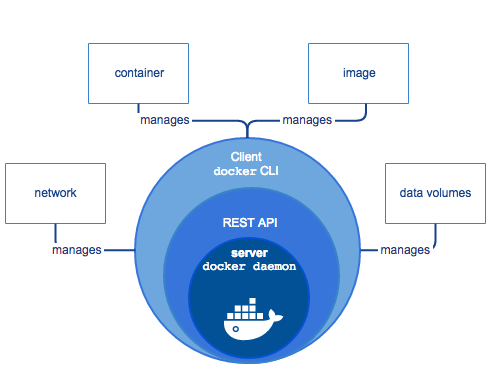
\includegraphics[width=0.8\textwidth]{figures/docker-engine.png}
    \caption{Estructura de Docker}
    \label{docker}
\end{figure}

Así, se puede decir que utilizar Docker multiplica exponencialmente la escalabilidad y portabilidad de una aplicación, ya que no hay que prestar atención el sistema operativo latente en el anfitrión, pues la infraestructura del contenedor configura el entorno que la aplicación necesita. Consideramos que esta característica puede resolver toda la parte de accesibilidad a la herramienta que queremos construir, en tanto que se pretende que ésta sea un cliente que se comunica con una aplicación robótica remota y que necesita disponer de ciertos recursos y ejecutar ciertas tareas en el sistema del usuario.

La necesidad de usar esta plataforma surgió a medida que avanzó el proyecto, dadas sus implicaciones de seguridad, principalmente, y en segunda instancia debido a que la usabilidad de una herramienta reside en gran medida en que el proceso de instalación y puesta a punto de la misma no sea tedioso y, si es posible, inexistente, además del hecho de que eliminar la necesidad de instalación supone que el rango de potenciales usuarios se amplia hasta prácticamente cualquiera, ya que se pasa a no depender del sistema ni del entorno del usuario. Por tanto, persiguiendo las ventajas de un proyecto multiplataforma e independiente del sistema del cliente, investigamos Docker para mejorar la experiencia de usuario al evitar que éste tenga que llevar a cabo procesos de instalación, en tanto que podríamos disponer uno con todo lo necesario para que el cliente disfrute de las funciones para aplicaciones robóticas que pueda necesitar desde un entorno predispuesto y debidamente configurado a través de un contenedor.

\subsection{Simulador Gazebo}

Gazebo\footnote{\url{http://gazebosim.org/}} es un simulador cuyo uso está muy extendido en el campo de la robótica. Para poder evaluar el código destinado a un robot o sistema en un paso previo al de cargar dicho código en él, este simulador ofrece la capacidad de emular diversos escenarios tridimensionales customizables para robots autónomos. Esta diseñado para probar lógica de elusión de objetos y algoritmos de visión artificial, aunque su uso es extensible a cualquier tipo de implementación. 

Para nuestro proyecto era necesario disponer de soporte de simulación, dado que la intención es ofrecer un interfaz que funcione con robots reales y simulados para ofrecer la robótica a usuarios con y sin recursos. Además, especialmente en un proceso de aprendizaje o investigación en el que no se es experto en la materia tratada, se hace necesario probar el \textit{software} desarrollado antes de correr el riesgo de utilizarlo en un sistema real, que suele ser frágil y costoso en este campo, e incluso peligroso para los usuarios según el diseño mecánico del sistema y la tarea a realizar. El uso de simuladores en robótica evita la implementación de costosas y poco útiles pruebas de código en \textit{hardware} real en las primeras fases del desarrollo. Ofrecer este ``\textit{hardware} virtual'' permite evaluar y supervisar el desempeño de la lógica en todo momento, agilizando el desarrollo y abaratando costes, y abre el abanico de usuarios que pueden acceder a la robótica. Estas son las razones principales bajo su elección como simulador para este proyecto, además del hecho de que es de código abierto. Sin embargo, existen muchos otros simuladores con estas mismas características que hacen que Gazebo esté lejos del estándar de simulación robótica. A continuación veremos otras características que hemos analizado para elegir este y no otro en relación con el uso final que se va a hacer de él: docente, investigativo o formativo.

La característica más importante es su versatilidad, ya que puede simular robots, objetos y los sensores actuales más utilizados en entornos complejos de
interior y exterior con multitud de elementos realistas para los robots. Es de los pocos simuladores que quitan el foco de construir simulaciones realistas para los usuarios humanos e incluyen elementos que pueden emular problemas reales como ruido sensorial producido por superficies reflectantes, o la inclusión de texturas que el robot puede detectar, entre otras cosas. Además, posee un interfaz de gran calidad.

Por otro lado cabe mencionar su robusto motor de físicas\footnote{\url{http://opende.sourceforge.net}} (Fig. \ref{gazebo-physics}), creado por Russel Smith, que permite caracterizar elementos del robot como su masa, el rozamiento al que se somete, su inercia, amortiguamiento, etc. Con ello y los mecanismos que proporciona para conectar los cuerpos entre sí formando relaciones cinemáticas y dinámicas, y las propiedades de color, textura y transparencia que se pueden incluir, se consigue diseñar modelos de simulación con visualizaciones muy realistas a través de OpenGL\footnote{\url{https://www.opengl.org/}} que se adaptan bien a situaciones reales (Fig. \ref{gazebo-models}).

\begin{figure}[!hbtp]  \centering\noindent
    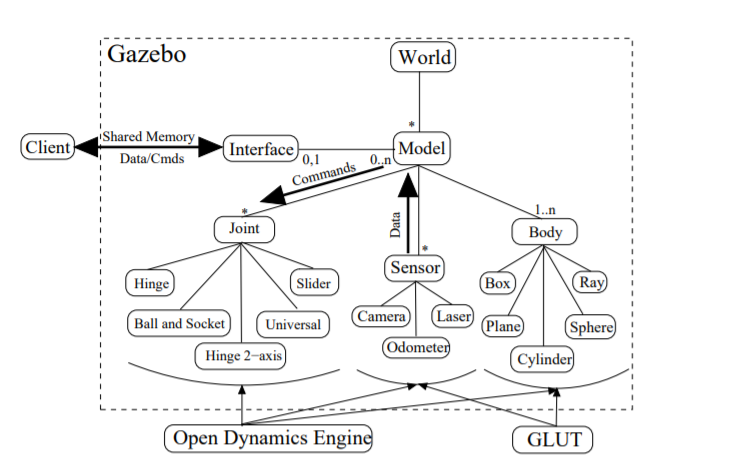
\includegraphics[width=0.99\textwidth]{figures/gazebo-engine.png}
    \caption{Motor de físicas de Gazebo}
    \label{gazebo-physics}
\end{figure}

\begin{figure}[!hbtp]  \centering\noindent
    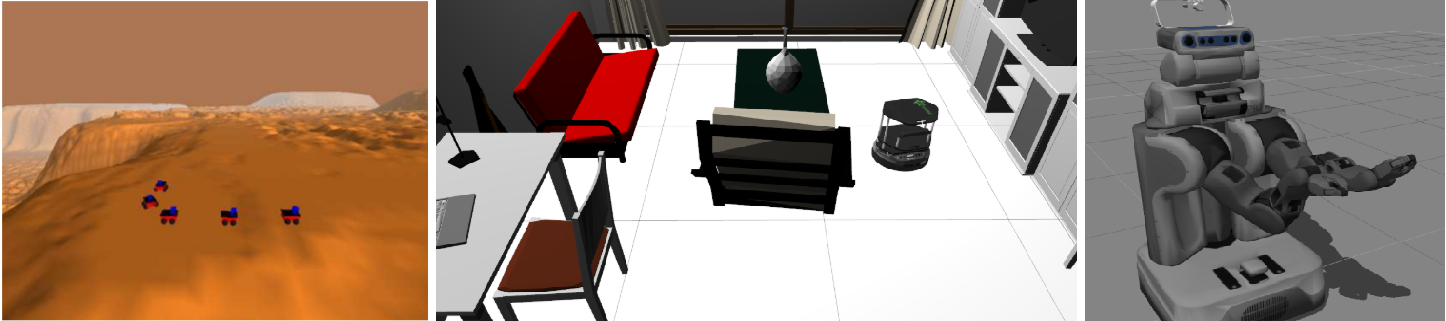
\includegraphics[width=0.99\textwidth]{figures/gazebo-models.png}
    \caption{Modelos de Simulación en Gazebo}
    \label{gazebo-models}
\end{figure}
 
La configuración de mundos 3D con Gazebo se describe en ficheros con extensión ``\textit{.world}'', que son documentos de texto en formato de marcado XML (\textit{Extensible Markup Language}) de documentos, con etiquetas definidas en el lenguaje \textit{Simulation Description Format} (SDF), donde se
recogen todos los elementos del escenario (luz ambiente, propiedades del cielo, sombras, conjunto de modelos, \textit{plugins}, propiedades
físicas y temporales etc.).
 
Aunque la versión 7 de Gazebo incluy eun editor de modelos muy básico con el que se pueden crear robots y mundos simples, el simulador acepta la importación de modelos complejos creados con programas de modelado como Blender o Sketchup. A partir del modelo, se especifica un \textit{plugin} asociado al mismo para recoger y publicar la información de los sensores, y para enviar órdenes a los actuadores y dotar al robot de inteligencia e interacción. Es aquí donde existe la relación entre el simulador y el sistema de comunicaciones de ROS, que hará las funciones de mediador entre la aplicación y el robot simulado en este caso.

\subsection{Framework Django}

Para testar la herramienta que queremos construir, necesitamos una aplicación robótica que se conecte a ella y que ofrezca cierto servicio robótica, en nuestro caso orientado hacia la docencia o investigación. Este servicio debe usar el API que la ``Ejecución mixta'' proporcionará para montar el servicio sobre los mecanismos que se incluirán en el contenedor Docker del que dispondrá el cliente. Así, la aplicación remota ofrecerá la funcionalidad para la que ha sido diseñada sin consumir recursos en el sistema anfitrión, y llevará a cabo el proceso de ``Ejecución mixta'' que queremos conseguir para garantizar el acceso a cualquier cliente. Esta aplicación remota será construida a través de Django.

Django\footnote{\url{https://www.djangoproject.com/}} es un marco de trabajo clasificado como tecnología de servidor de alto nivel en Python que garantiza el desarrollo rápido del lado servidor de una aplicación y su diseño. Ofrece gran cantidad de funcionalidad resuelta que se encarga de las molestias del desarrollo Web, por lo que se puede construir una aplicación reutilizando módulos de código con la funcionalidad típica de una aplicación, de tal manera que el desarrollo puede centrarse en escribir la lógica específica del servicio que quiere ofrecer sin necesidad de empezar desde el principio programando cada módulo. Es gratuito y de filosofía abierta.

La arquitectura de Django resulta bastante simple. Como se puede ver en la Figura \ref{django}, organiza la aplicación de tal manera que resulta muy sencillo conocer en todo momento el estado del proceso de servicio.

\begin{figure}[!hbtp]  \centering\noindent
    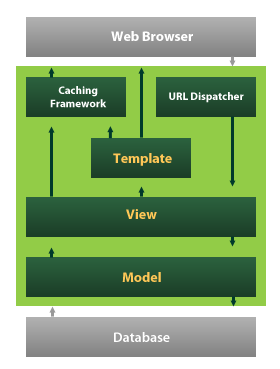
\includegraphics[width=0.65\textwidth]{figures/django-arch.png}
    \caption{Arquitectura de Django}
    \label{django}
\end{figure}

Se controla muy fácilmente lo que el usuario ve a través de las vistas de Django, con las que además se dota a la aplicación web de dinamismo e inteligencia. También se controla cómo ve el usuario el contenido de la aplicación a través de las plantillas, que proporcionan herramientas de interacción entre el usuario y el servidor y le permiten realizar peticiones simples para potenciar la funcionalidad que se puede ofrecer. Por último facilita mecanismos muy simples de gestión y acceso a bases de datos a través de distintas tecnologías como MySQL o MongoDB, necesarias para las aplicaciones y que evita la especialización en lenguajes utilizados para peticiones a bases de datos por parte del desarrollador. En resumen, facilita el proceso de construcción y diseño de aplicaciones web para que el desarrollador no tenga que preocuparse por el bajo y medio nivel.

Esta característica, junto con la escalabilidad del lado servidor construido con tecnologías web de servidor, es precisamente la que decantó la balanza hacia el uso de Django para la aplicación con la que testar nuestra herramienta, ya que construir una aplicación robótica no es el foco ni el objetivo de este trabajo, sino que es una tarea secundaria necesaria para demostrar la ``Ejecución mixta''.

\subsection{Biblioteca OpenCV}
En primera instancia, la herramienta que planeábamos diseñar perseguía la ampliación del acceso al campo de la Visión Artificial de la robótica, en tanto que los sensores necesarios (cámaras, ToF, sensores de profundidad) son los más extendidos entre los usuarios de cualquier clase. Es por eso que, aunque la funcionalidad finalmente se extendió para que la herramienta soportase cualquier ámbito de la ciencia robótica, merece una mención especial la tecnología utilizada para el control de los sensores de imagen: las bibliotecas OpenCV\footnote{\url{https://opencv.org/}}.

OpenCV es una librería de código abierto desarrollada por Intel y publicada bajo licencia BSD. Incluye gran variedad de herramientas para el tratamiento digital de la imagen y el aprendizaje máquina. Su propósito principal es facilitar la programación de aplicaciones en tiempo real de visión por computador mediante la disposición de módulos de lógica resuelta que implementan alguna técnica de procesamiento o análisis de la imagen (Fig. \ref{opencv}).

\begin{figure}[!hbtp]  \centering\noindent
    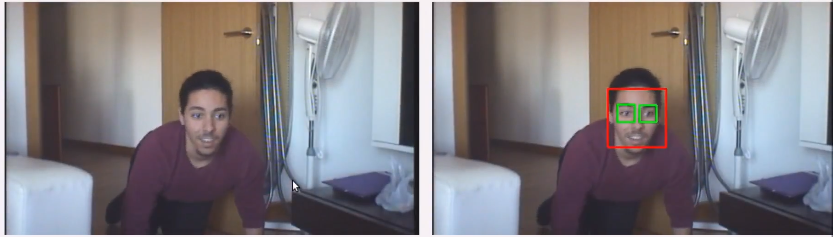
\includegraphics[width=0.99\textwidth]{figures/opencv-face.png}
    \caption{Herramientas de procesado con OpenCV: Segmentación de caras.}
    \label{opencv}
\end{figure}

Se escogió esta librería por ser el estándar en lo relativo a la visión artificial, y se usará tanto para obtener acceso al \textit{hardware} que proporcione la fuente de imágenes como para utilizarse en la aplicación robótica que se creará para tratar las matrices de información 2D.

\subsection{Lenguajes de Programación: Python, JavaScript}

En cuanto a los lenguajes de programación escogidos para la implementación, se hace necesaria una sub-división en dos ámbitos:

\begin{itemize}
    \item Lenguaje de Aplicación y de Usuario. Es necesario escoger un lenguaje para programar toda la lógica de la aplicación a ofrecer. También se hizo necesario ofrecer un lenguaje al cliente de la aplicación para que aborde su desarrollo robótico.
    \item Lenguaje de Infraestructura. El contexto de tecnologías web en el que se encuentra la ``Ejecución Mixta'' requiere de la elección de un lenguaje que pueda hacer que los distintos agentes colaboren entre sí, principalmente mediante protocolos.
\end{itemize}

Así, el primer lenguaje escogido ha sido Python\footnote{\url{https://www.python.org/}}, como lenguaje de aplicación y usuario. En primer lugar, la elección se debe a la compatibilidad del lenguaje con la infraestructura detallada en este capítulo. Tanto Gazebo como ROS, OpenCV, Jupter y Django ofrecen interfaces Python. Por otro lado están las atractivas características del lenguaje, como sus estructuras de datos integradas de alto nivel, su apariencia intuitiva, y la combinación del tipado y el enlace dinámicos, que hacen al lenguaje idóneo para desarrollar aplicaciones rápidamente. Además, su sintaxis resulta simple y fácil de aprender y enfatiza la legibilidad, lo que a grandes rasgos reduce el costo del mantenimiento del programa. Además fomenta la modularidad del programa y la reutilización de código, lo que lo convierte en un lenguaje de programación muy adecuado para el aprendizaje. Eliminando las peculiaridades que pueden hacer a un lenguaje difícil de tratar, conseguimos que el usuario se centre en su objetivo de carácter robótico y evite los dilemas y contratiempos relacionados con la programación.

En cuanto al lenguaje a usar para la infraestructura de la herramienta, el entorno web hace que la elección de JavaScript\footnote{\url{https://developer.mozilla.org/es/docs/Web/JavaScript}} resulte prácticamente obvia. Desde el 2012, todos los navegadores modernos soportan completamente ECMAScript 5.1\footnote{\url{https://developer.mozilla.org/en-US/docs/Web/JavaScript/Language_Resources}}, el estándar de JavaScript. Por tanto, este lenguaje nos va a permitir realizar actividades complejas en páginas web, entorno en el que deberá operar la ``Ejecución Mixta'' para aplicaciones robóticas. Este entorno nos permitirá aprovecharnos de los mecanismos y protocolos de comunicación de Internet para resolver el intercambio de mensajes entre nuestra herramienta, la aplicación robótica, el navegador y el cliente.

\section{Infraestructura de la Aplicación}

En esta sección abordaremos la relación existente entre las herramientas seleccionadas y descritas anteriormente y comentaremos el diseño final de la herramienta, así como la jerarquía establecida.

\begin{figure}[!ht]  \centering\noindent
    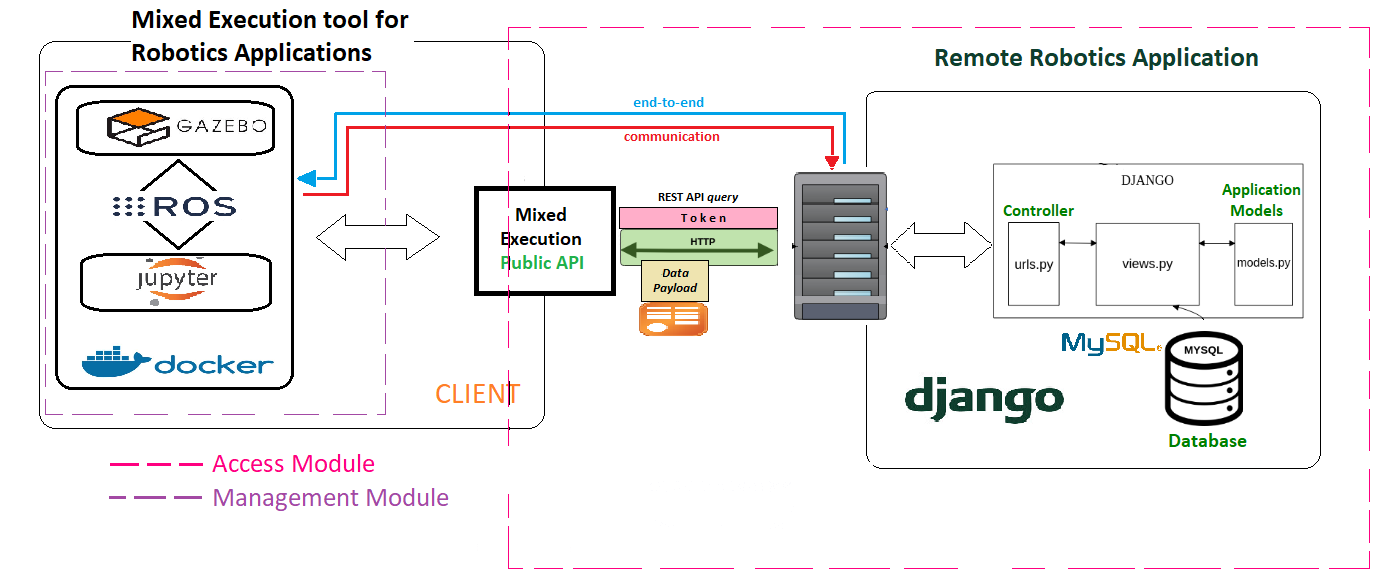
\includegraphics[width=1.20\textwidth,height=10cm]{figures/ejecucion-mixta-infograma.png}
    \caption{Arquitectura de la Ejecuión Mixta para Aplicaciones de Robótica.}
    \label{mixedexecarch}
\end{figure}

Se puede ver en el infograma (Fig. \ref{mixedexecarch}) que la solución ideada para la ``Ejecución Mixta'' se divide claramente en dos módulos, cada uno sub-dividido a su vez en una serie de capas encargadas de una parte específica del proceso:

\begin{itemize}
    \item [\textbullet] El primero de ellos es el \textbf{módulo de acceso}. Este módulo será el encargado de dirigir la comunicación entre el lado servidor y el lado cliente de la aplicación para que se produzca la ``Ejecución Mixta''. Organizará ambas partes y actuará como un secuenciador que decidirá en cada momento quién lleva el peso de la comunicación. Su propósito principal será el de garantizar el acceso a la herramienta.
    \item [\textbullet] El otro es el \textbf{módulo de gestión}. Estará recubierto por un API público que permitirá a las aplicaciones externas realizar la conexión y aprovechar las funciones de ``Ejecución Mixta'' para ofrecer un servicio. Será el encargado de redirigir cada petición y respuesta de la aplicación al proceso que corresponda de forma segura, dentro de la ejecución del cliente.
\end{itemize}

Dada la clara distinción entre las distintas sub-tareas que realiza cada módulo, consideramos adecuado bajar otro escalón en cuanto a la arquitectura, y dividir cada módulo en capas encargadas de tareas sencillas, sobre las que se pudiese construir de manera modular. 

\subsection{Capa de Aplicación}

\begin{figure}[!hbtp]  \centering\noindent
    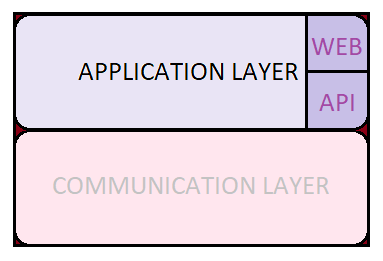
\includegraphics[width=0.6\textwidth]{figures/layer4.png}
    \caption{Módulo de Acceso: Capa de Aplicación}
    \label{layer4}
\end{figure}

La capa de aplicación tendrá la tarea específica de emparejar la funcionalidad que ofrece la aplicación remota como servicio con la información que necesita de la ejecución en el lado cliente para dar soporte a dicha funcionalidad. Requerirá de la intervención de dos agentes para cumplir su tarea:

\begin{itemize}
    \item [--] Será necesario que la aplicación robótica que se ofrece a través de la web que quiere beneficiarse de la ``Ejecución Mixta'' inicie la conexión con el cliente remoto, en calidad de cliente de ``Ejecución Mixta''. Esto es así dada la naturaleza de la información a la que más tarde pedirá acceso, la cual se genera completamente en el cliente durante la ejecución y pondrá a disposición de quien la solicite. El cliente de la aplicación hace las funciones de servidor de la herramienta, ya que está pensada para ser colocada en el lado del cliente web.
    \item [--] Con la conexión iniciada, esta capa debe solicitar la información que necesite al servidor de ``Ejecución Mixta'', en tiempo de ejecución, para que la aplicación funcione como se espera. Esta solicitud se realizará a través del API de ``Ejecución Mixta''.
\end{itemize}

Así, el mecanismo completo de la capa de aplicación comenzará por establecer la conexión con la herramienta, utilizando uno o varios \textit{endpoints} en función de los canales de comunicación que se quiera establecer para recopilar la información necesaria y generará un comando específico para configurar en la herramienta el tipo de enlace que se requiere y el conjunto de herramientas que se necesita para la ejecución.

\begin{lstlisting}[language=bash, caption=Comando de configuración de Ejecución Mixta]

mkdir -p /tmp/siguelineaIR/ && docker run --rm -e DISPLAY=:0
-e JDEROBOT_SIMULATION_TYPE=REMOTE --entrypoint 
/entrypoint_mixed_execution.sh -v 
/tmp/siguelineaIR:/home/jderobot/volume/user/exercise:rw 
-p 8888:8888 -p 8080:8080 -p 9001:9001 -p 9002:9002 
-it tfmdocker/local:dev f1_1_simplecircuit.launch

\end{lstlisting}


\subsection{Capa de Comunicación}

\begin{figure}[!hbtp]  \centering\noindent
    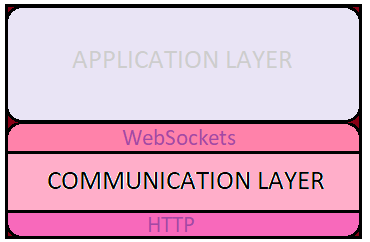
\includegraphics[width=0.6\textwidth]{figures/layer3.png}
    \caption{Módulo de Acceso: Capa de Comunicación}
    \label{layer3}
\end{figure}

Encargada del establecimiento de los canales de comunicación entre la aplicación robótica externa y la herramienta de ``Ejecución Mixta'' una vez iniciada la conexión. Se utilizará principalmente el protocolo HTTP para la comunicación que tiene lugar a través de Internet y que pretende conectar la herramienta y la capa de aplicación. El formato de los mensajes intercambiados será similar al de un REST API basado en solicitudes y respuestas HTTP utilizando los métodos clásicos: GET, POST, PUT, DELETE y OPTIONS.

Adicionalmente se utilizará un medio WebSockets para el intercambio de mensajes ligeros, más relacionados con el interfaz de usuario de la aplicación y aquella información que requiere un refresco de carga ligera pero constante. Se utilizará también como canal auxiliar para la información que necesiten enviar los agentes y procesos en ejecución durante la ``Ejecución Mixta'', en caso de necesitarse.

\subsection{Capa de Seguridad}

\begin{figure}[!hbtp]  \centering\noindent
    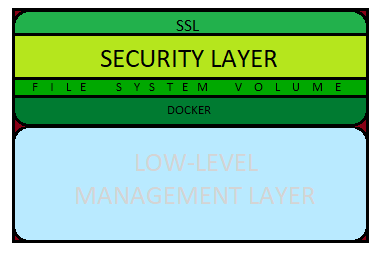
\includegraphics[width=0.6\textwidth]{figures/layer2.png}
    \caption{Módulo de Gestión: Capa de Seguridad}
    \label{layer2}
\end{figure}

Debemos distinguir dos niveles de seguridad en el proceso de ``Ejecución Mixta'':

\begin{itemize}
    \item [--] En primer lugar, hay que garantizar la fiabilidad e integridad de los mensajes intercambiados con la herramienta. Al ser tanto HTTP como WebSockets dos protocolos en los que la información viaja en claro, como texto plano, por el canal de comunicación, decidimos incluir una capa que garantiza seguridad a través del protocolo SSL, que también asegurará que los mensajes no se corrompan. Este nivel tiene un grado bajo de criticidad.
    \item [--] Por otro lado, existe un alto riesgo cuando se trata de permitir que un código cuya fuente es externa se ejecute en nuestro sistema. Esto es precisamente lo que se pretende hacer con esta herramienta, de manera que se debe asegurar que, sea cual sea la fuente del código y su contenido, los problemas de seguridad se pueden contener, evitando que actúen sobre el sistema del cliente, el cual lleva a cabo la ejecución. Para esto utilizaremos la plataforma Docker.
\end{itemize}

Para mantener segura la conexión entre cliente y servidor de ``Ejecución Mixta'' y entre cliente y servidor web a través de Internet utilizamos el protocolo TLS a Nivel de Transporte según la clasificación OSI, que asigna una serie de certificados SSL basados en criptografía asimétrica a cada agente de la comunicación para ser autenticados a la hora de intercambiarse la clave simétrica con la cual se pueden decodificar los datos intercambiados, que viajan encriptados en todo momento. Así funcionan la mayoría de sitios web en la actualidad.

El mayor peso en cuanto a seguridad recae sobre la tarea para la que ha sido diseñada la herramienta. El código que proviene del servidor web puede no ser de confianza o de dudosas intenciones, por lo que no se puede permitir a la ligera su ejecución en la máquina del cliente, dado que esto podría conllevar graves riesgos de pérdida de datos (mediante instrucciones de borrado de disco que viajasen en el código), malfuncionamientos y ataques de toda clase. Por ello, se ha montado lo que se denomina ``volumen'' (Fig. \ref{volumen}) sobre el sistema de ficheros local del servidor de ``Ejecución Mixta'' (cliente web), y se ha restringido el acceso del contenedor Docker y de las instrucciones que en él se ejecutan a este volumen, impidiendo en todo caso que cualquier suceso tenga consecuencias o repercusiones fuera de él. 

\begin{figure}[!hbtp]  \centering\noindent
    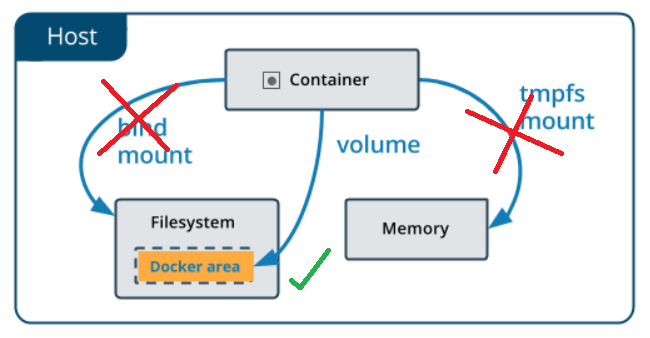
\includegraphics[width=0.75\textwidth]{figures/volumen.png}
    \caption{Volumen de Docker}
    \label{volumen}
\end{figure}

Se puede ver un volumen como una forma de almacenar datos persistentes en el sistema de ficheros local del cliente, necesario para gestionar el acceso al \textit{hardware} entre otras cosas para esta herramienta, que permanece completamente aislado de la funcionalidad central y el \textit{core} de la máquina anfitriona. Esto significa que el contenedor sólo podrá actuar sobre el contenido del volumen y no sobre el contenido externo, pero se podrá beneficiar de todas las ventajas que ofrece el administrador del sistema de archivos del sistema operativo del usuario. Así, aún en el supuesto de que se tratase de utilizar la ``Ejecución Mixta'' en conjunto con una aplicación robótica maliciosa (supuesto muy improbable), el mayor daño posible que se podría causar se reduciría a parar y reiniciar el contenedor, eliminándose todo indicio de código maligno o sospechoso.

\subsection{Capa de Bajo Nivel}

\begin{figure}[!hbtp]  \centering\noindent
    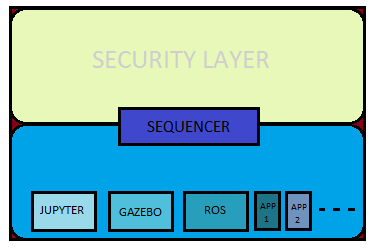
\includegraphics[width=0.6\textwidth]{figures/layer1.png}
    \caption{Módulo de Gestión: Capa de Gestión del Bajo Nivel}
    \label{layer1}
\end{figure}

La capa de menor nivel y mayor grado de restricción de la herramienta es la que hemos denominado Capa de Bajo Nivel, cuya puerta es sólo visible para el secuenciador del módulo de gestión. 

Una vez resuelta la comunicación y superada la seguridad, el motor de la ``Ejecución Mixta'' debe decidir qué se necesita en todo momento según las peticiones que recibe, y más importante, a quién redirige cada mensaje. Para la Capa de Comunicación, todos los mensajes tienen el mismo destinatario, en función de la conexión HTTPS que se abre para comunicar el lado servidor y el cliente. Este receptor único es un módulo secuenciador, configurado y levantado a través de un \textit{entrypoint} que activará en cada momento la aplicación, herramienta o plataforma auxiliar que se necesite para satisfacer las peticiones de la aplicación robótica, y organizará el canal de bajo nivel para que no se produzcan colisiones durante el proceso. La forma de gestionar la secuenciación se basa en la apertura de nuevos sub-canales de comunicación, ya en un entorno puramente local o \textit{localhost}, y en una redirección de la información obtenida en cada sub-canal hacia el canal HTTPS principal, formateando cada paquete de información según su fuente, su destinatario en la aplicación robótica y su prioridad, a través de cabeceras y estructuras de datos JSON fácilmente procesables por una aplicación web, y accesibles a través del API público de la Capa de Aplicación (Figs. \ref{nb_put_req} y \ref{exec_req}).

\begin{lstlisting}[language=bash, caption=Ejemplo de la parte HTTP de los mensajes]
PUT /api/contents/descarga_bundle.png HTTP/1.1
Host: 127.0.0.1:8888
Connection: keep-alive
Content-Length: 25899
Sec-Fetch-Mode: cors
Origin: http://localhost:8000
User-Agent: Mozilla/5.0 (X11; Linux x86_64) AppleWebKit/537.36
(KHTML, like Gecko) Chrome/77.0.3865.120 Safari/537.36
Content-Type: application/json
Accept: */*
Sec-Fetch-Site: cross-site
Referer: http://localhost:8000/local
Accept-Encoding: gzip, deflate, br
Accept-Language: es-ES,es;q=0.9
\end{lstlisting}

\begin{figure}[!hbtp]  \centering\noindent
    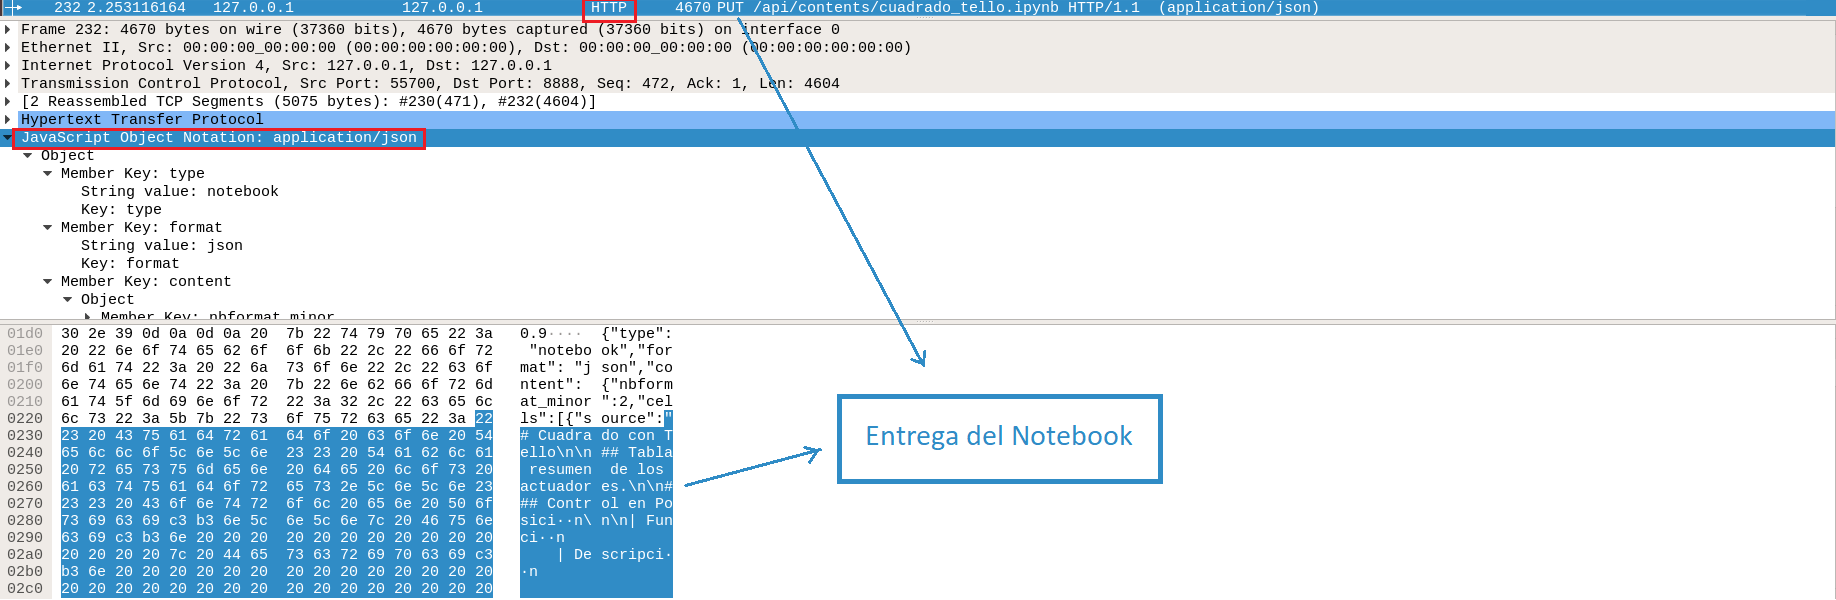
\includegraphics[width=1.05\textwidth]{figures/notebook_put_request.png}
    \caption{Mensaje de Entrega del Cuadernillo o Notebook}
    \label{nb_put_req}
\end{figure}

\begin{figure}[!hbtp]  \centering\noindent
    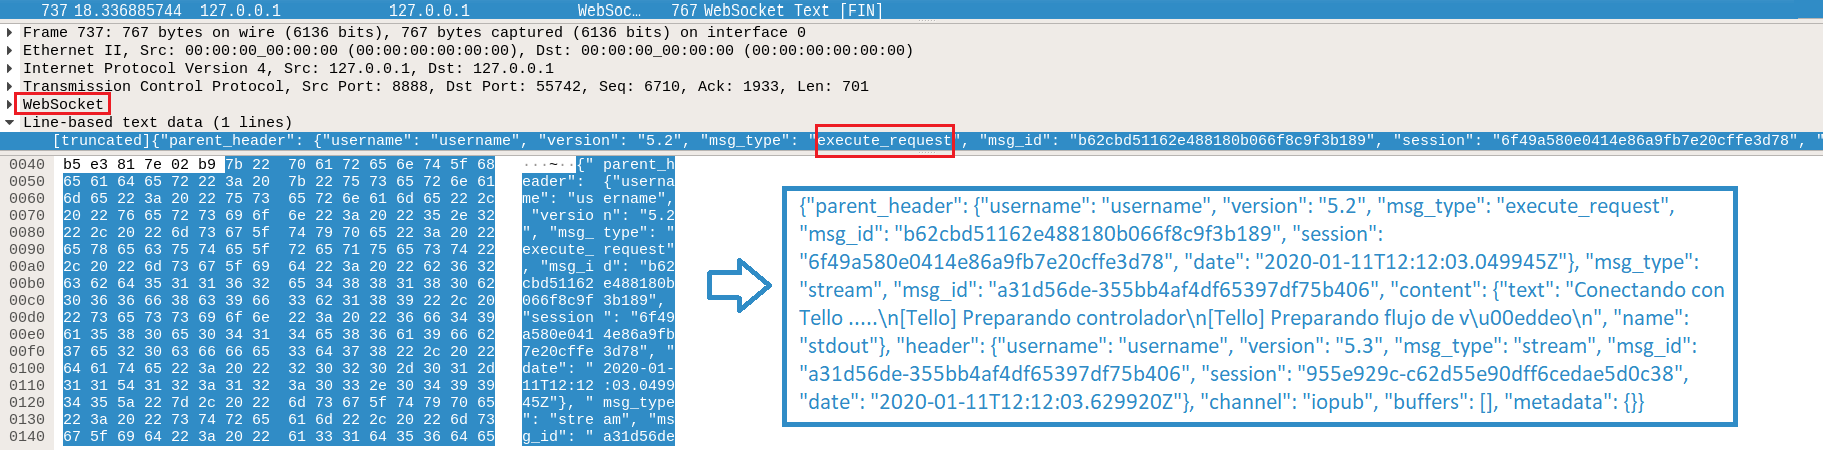
\includegraphics[width=1.05\textwidth]{figures/execute_request.png}
    \caption{Mensaje de Respuesta de Petición de Ejecución }
    \label{exec_req}
\end{figure}

Además, los diferentes programas que ejecutan en el interior del contenedor Docker en el servidor de ``Ejecución mixta'' necesitan un mecanismo de intercomunicación de tipo p2p, sin pasar por todo el mecanismo de transmisión, recepción y procesado descrito anteriormente como parte de la arquitectura, para facilitar la colaboración entre ellos sin sucumbir a problemas de tipo \textit{jitter}, grandes retardos de extremo a extremo o pérdidas de información y largas esperas de reenvios que caracterizan a muchos enlaces de Internet basados en TCP/IP. Para implementar este mecanismo de comunicación interna aprovecharemos las herramientas de ROS, donde el secuenciador tendrá el rol de \textit{MASTER} y las diferentes plataformas y aplicaciones en ejecución actuarán como suscriptores y publicadores de información a través de \textit{topics} conocidos por todos. Así, se dispondrá por ejemplo un HAL API (\textit{Hardware Abstraction Layer}) que permitirá a todos los programas que lo requieran el acceso a las interfaces de sensado y actuación del robot, ya sea real (con \textit{plugins} y \textit{drivers} reales involucrados) o simulado (con \textit{drivers} virtuales). Este método de intercomunicación facilita el crecimiento de la red de agentes (que simplemente ``escuchan'' la información del canal que les conviene y publican los datos que generan que pueden resultar útiles para otros procesos) que se puede lanzar para proporcionar mayor volumen de información a la aplicación robótica remota, y por tanto a la construcción de aplicaciones remotas más ricas que no produzcan carga computacional en el lado servidor de la misma gracias a la ``Ejecución Mixta''.